% Gabarit pandoc des corrigés publiés (brut et guidé). Contenu sans marque ni nom de site.
% Compilation : lualatex (latexmk -lualatex).
% Le Markdown reste la source unique : ne pas éditer ce fichier .tex à la main.
\documentclass[11pt,a4paper]{article}

% --- Moteur, polices (Latin Modern) et langue ---------------------------------
\usepackage{iftex}
\ifLuaTeX\else\errmessage{Ce document se compile avec lualatex}\fi
\usepackage{amsmath,amssymb,mathtools}
\usepackage{fontspec}
% mathrm=sym : \mathrm prend ses glyphes dans la police mathématique (ℓ, μ, Ω), comme KaTeX.
\usepackage[math-style=TeX,bold-style=TeX,mathrm=sym]{unicode-math}
% Repli pour les glyphes absents de Latin Modern (indices et exposants Unicode,
% flèches, filets des schémas en texte, symboles) : DejaVu, puis Latin Modern Math
% (ℓ, lettres mathématiques Unicode des légendes).
\directlua{
  luaotfload.add_fallback("repliTexte", {"DejaVuSerif:mode=harf;", "DejaVuSans:mode=harf;", "file:latinmodern-math.otf:mode=harf;"})
  luaotfload.add_fallback("repliMono", {"DejaVuSansMono:mode=harf;", "DejaVuSans:mode=harf;", "file:latinmodern-math.otf:mode=harf;"})
}
\setmainfont{Latin Modern Roman}[RawFeature={fallback=repliTexte}]
\setsansfont{Latin Modern Sans}[RawFeature={fallback=repliTexte}]
\setmonofont{Latin Modern Mono}[RawFeature={fallback=repliMono}]
\setmathfont{Latin Modern Math}
\usepackage[french]{babel}
\frenchsetup{SmallCapsFigTabCaptions=false}

% --- Mise en page --------------------------------------------------------------
\usepackage[a4paper,margin=2.2cm,headheight=14pt,footskip=1.2cm]{geometry}
\usepackage{microtype}
\setlength{\emergencystretch}{4em}
\tolerance=1500
\setlength{\parindent}{0pt}
\setlength{\parskip}{0.55\baselineskip plus 2pt minus 1pt}
\usepackage{xcolor}
% Gris nommés : babel-french rend « ! » actif dans le document.
\definecolor{gris2}{gray}{0.98}
\definecolor{gris3}{gray}{0.97}
\definecolor{gris5}{gray}{0.95}
\definecolor{gris35}{gray}{0.65}
\definecolor{gris40}{gray}{0.60}
\definecolor{gris45}{gray}{0.55}
\definecolor{gris50}{gray}{0.50}
\definecolor{gris55}{gray}{0.45}
\definecolor{gris60}{gray}{0.40}
\definecolor{gris65}{gray}{0.35}
\definecolor{gris70}{gray}{0.30}
\definecolor{gris80}{gray}{0.20}
\definecolor{gris85}{gray}{0.15}
\usepackage{graphicx}
\usepackage{float}
\usepackage{caption}
\captionsetup{font=small,labelformat=empty,justification=centering}
\usepackage{booktabs,longtable,array,multirow,calc}
\usepackage{siunitx}
\sisetup{locale=FR}
\usepackage[version=4]{mhchem}
\usepackage{listings}
\usepackage{fancyhdr}
\usepackage{lastpage}
\usepackage[most]{tcolorbox}
\usepackage{enumitem}
\setlist{nosep,leftmargin=*,topsep=2pt}
\usepackage[hidelinks,unicode]{hyperref}
\usepackage{bookmark}
\hypersetup{pdftitle={X-ENS MP-PC-PSI — Informatique B 2026},pdfauthor={Rédigé par IA},pdfcreator={LaTeX},pdfsubject={Corrigé brut}}
\usepackage{xurl}

% --- Pandoc : listes, tableaux, figures ----------------------------------------
\providecommand{\passthrough}[1]{#1}
\providecommand{\tightlist}{\setlength{\itemsep}{0pt}\setlength{\parskip}{0pt}}

\makeatletter
\def\maxwidth{\ifdim\Gin@nat@width>\linewidth\linewidth\else\Gin@nat@width\fi}
\def\maxheight{\ifdim\Gin@nat@height>0.55\textheight 0.55\textheight\else\Gin@nat@height\fi}
\makeatother
\setkeys{Gin}{width=\maxwidth,height=\maxheight,keepaspectratio}
\setcounter{secnumdepth}{-\maxdimen}
\providecommand{\pandocbounded}[1]{#1}
\usepackage{longtable,booktabs,array}

% --- Code (listings) -----------------------------------------------------------
\lstset{
  basicstyle=\ttfamily\small,
  columns=fullflexible,
  keepspaces=true,
  breaklines=true,
  breakatwhitespace=false,
  postbreak=\mbox{\textcolor{gris50}{$\hookrightarrow$}\space},
  frame=single,
  rulecolor=\color{gris35},
  framesep=4pt,
  xleftmargin=5pt,xrightmargin=5pt,
  backgroundcolor=\color{gris3},
  keywordstyle=\bfseries,
  commentstyle=\color{gris65},
  stringstyle=\color{gris80},
  showstringspaces=false,
  tabsize=4,
  extendedchars=true,
  aboveskip=6pt,belowskip=6pt,
}

% --- Macros des corrigés (KaTeX ↔ LaTeX) ---------------------------------------
% Les corrigés sont écrits pour KaTeX : on définit ici ce que KaTeX connaît et
% que LaTeX n'a pas, sans jamais retoucher le Markdown.
\providecommand{\R}{\mathbb{R}}
\providecommand{\N}{\mathbb{N}}
\providecommand{\Z}{\mathbb{Z}}
\providecommand{\Q}{\mathbb{Q}}
\providecommand{\C}{\mathbb{C}}
\providecommand{\dd}{\mathrm{d}}
\providecommand{\llbracket}{\lBrack}
\providecommand{\rrbracket}{\rBrack}
\providecommand{\lBrace}{\lbrace}
\providecommand{\rBrace}{\rbrace}
\providecommand{\Box}{\square}
\providecommand{\Diamond}{\lozenge}
\providecommand{\varnothing}{\emptyset}
\providecommand{\argmax}{\operatorname*{arg\,max}}
\providecommand{\argmin}{\operatorname*{arg\,min}}
\renewcommand{\leq}{\leqslant}
\renewcommand{\geq}{\geqslant}

% Équation hors texte : réduite à la largeur de la ligne si elle déborde.
\newsavebox{\boiteequation}
\newcommand{\equationajustee}[1]{%
  \sbox{\boiteequation}{$\displaystyle #1$}%
  \ifdim\wd\boiteequation>\linewidth
    \[\resizebox{\linewidth}{!}{\usebox{\boiteequation}}\]%
  \else
    \[#1\]%
  \fi}

% --- Encadrés pédagogiques (sobres, lisibles en noir et blanc) -----------------
\tcbset{
  encadre/.style={
    enhanced,breakable,sharp corners,
    colback=white,colframe=gris55,
    boxrule=0.4pt,leftrule=2.2pt,
    left=6pt,right=6pt,top=3pt,bottom=3pt,
    before skip=6pt,after skip=6pt,
    fonttitle=\bfseries\small,coltitle=black,
    attach title to upper,after title={\quad},
    parbox=false,
  }
}
\newtcolorbox{indication}[1]{encadre,colframe=gris45,colback=gris2,title={Indication~#1}}
\newtcolorbox{methode}{encadre,colframe=gris70,title={Méthode}}
\newtcolorbox{piege}{encadre,colframe=gris85,boxrule=0.8pt,leftrule=2.2pt,title={Piège}}
\newtcolorbox{jury}{encadre,colframe=gris60,colback=gris5,title={Jury}}
\newtcolorbox{encadrenote}{encadre,colframe=gris40}

% --- Titres de section ---------------------------------------------------------
\usepackage{titlesec}
\titleformat{\section}{\Large\bfseries}{}{0pt}{}
\titleformat{\subsection}{\large\bfseries}{}{0pt}{}
\titleformat{\subsubsection}{\normalsize\bfseries}{}{0pt}{}
\titlespacing*{\section}{0pt}{14pt plus 4pt minus 2pt}{6pt}
\titlespacing*{\subsection}{0pt}{10pt plus 3pt minus 2pt}{4pt}
\titlespacing*{\subsubsection}{0pt}{8pt plus 2pt minus 2pt}{2pt}

% --- En-tête et pied de page ---------------------------------------------------
\pagestyle{fancy}
\fancyhf{}
\fancyhead[L]{\small\textsc{Corrigé brut} · X-ENS MP-PC-PSI}
\fancyhead[R]{\small Informatique B 2026}
\fancyfoot[L]{\footnotesize Corrigé rédigé par IA, non officiel}
\fancyfoot[R]{\footnotesize \thepage\,/\,\pageref*{LastPage}}
\renewcommand{\headrulewidth}{0.4pt}
\renewcommand{\footrulewidth}{0pt}
\fancypagestyle{plain}{\fancyhf{}\fancyfoot[R]{\footnotesize \thepage\,/\,\pageref*{LastPage}}\fancyfoot[L]{\footnotesize Corrigé rédigé par IA, non officiel}\renewcommand{\headrulewidth}{0pt}}

\begin{document}
\thispagestyle{plain}
\begin{center}
  {\small\scshape Corrigé brut}\par\smallskip
  {\LARGE\bfseries X-ENS MP-PC-PSI — Informatique B 2026\par}\medskip
  {\large X-ENS · MP-PC-PSI · Informatique B · 2026\par}
\end{center}
\vspace{2pt}\hrule\vspace{8pt}

\emph{Corrigé rédigé par IA, non officiel. Signalez toute erreur.}

Sujet : « Cycles et unification ». Durée 2 h, calculatrice interdite. Notations : \(s\rightsquigarrow t\) signifie qu'il existe un chemin (éventuellement vide) de \(s\) à \(t\) ; on note \texttt{époque}, \texttt{sortie}, \texttt{présent}, \texttt{compteur} les variables globales de l'énoncé.

Rappel du graphe de la figure 1 (listes d'adjacence, l'étiquette d'un arc est son indice) :

\begin{lstlisting}
a : [c, d]    b : [d, c]    c : [X, Y]    d : [Y, X]
e : [W, Z]    W : [Z]       X : []        Y : []        Z : []
\end{lstlisting}

\hypertarget{partie-i.-duxe9tection-de-cycles}{%
\section{Partie I. Détection de cycles}\label{partie-i.-duxe9tection-de-cycles}}

\hypertarget{question-1}{%
\subsection{Question 1}\label{question-1}}

Avec \texttt{présent\ =\ 1} et \texttt{compteur\ =\ 0}, l'appel \texttt{pp(\textquotesingle{}a\textquotesingle{})} se déroule ainsi :

\begin{itemize}
\tightlist
\item
  visite de \texttt{a}, puis de \texttt{c} ;
\item
  visite de \texttt{X} (sortie 0), puis de \texttt{Y} (sortie 1), fin de \texttt{c} (sortie 2) ;
\item
  visite de \texttt{d}, dont les deux cibles \texttt{Y} et \texttt{X} portent déjà l'époque 1, fin de \texttt{d} (sortie 3) ;
\item
  fin de \texttt{a} (sortie 4).
\end{itemize}

Les sommets \texttt{b}, \texttt{e}, \texttt{W}, \texttt{Z} ne sont pas visités et gardent leurs valeurs initiales.

\begin{figure}[H]
\centering
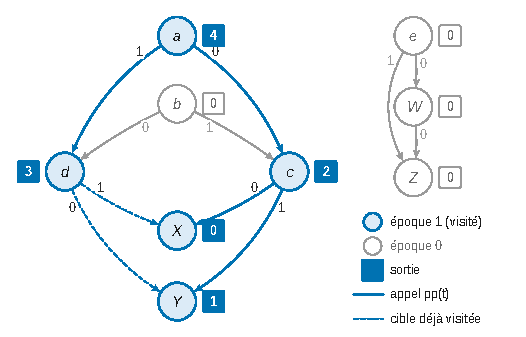
\includegraphics{figures/q01-parcours-pp-a.pdf}
\caption*{Figure 1 --- État des dictionnaires après pp(`a') : époque par le
remplissage, sortie dans la pastille, sur le graphe de la figure 1 du
sujet}
\end{figure}

\begin{longtable}[]{@{}llllllllll@{}}
\toprule\noalign{}
& a & b & c & d & e & W & X & Y & Z \\
\midrule\noalign{}
\endhead
\bottomrule\noalign{}
\endlastfoot
\texttt{époque} & 1 & 0 & 1 & 1 & 0 & 0 & 1 & 1 & 0 \\
\texttt{sortie} & 4 & 0 & 2 & 3 & 0 & 0 & 0 & 1 & 0 \\
\end{longtable}

\hypertarget{question-2}{%
\subsection{Question 2}\label{question-2}}

Les dictionnaires et \texttt{présent} sont quelconques, sous la seule hypothèse que les invariants sont vrais. Soit \(p\) la valeur de \texttt{présent} avant l'incrémentation. On est hors de \texttt{pp}, donc A2 est vrai : \(\texttt{\text{époque}}[t]\le p\) pour tout sommet \(t\).

Après l'incrémentation, \texttt{présent} vaut \(p+1\), et \texttt{époque} n'a pas changé. Donc

\equationajustee{\texttt{\text{époque}}[t]\le p<p+1=\texttt{\text{présent}},}

d'où \textbf{\(\texttt{\text{époque}}[t]\neq\texttt{\text{présent}}\) pour tout sommet \(t\)}.

\hypertarget{question-3}{%
\subsection{Question 3}\label{question-3}}

Pendant \texttt{pp(s)}, \texttt{présent} n'est pas modifié. Une époque n'est modifiée qu'à la ligne 16. Elle reçoit alors la valeur \texttt{présent}, sur un sommet visité, c'est-à-dire un sommet sur lequel \texttt{pp} est appelée. On montre que \textbf{les sommets visités sont exactement les sommets accessibles depuis \(s\)}.

\emph{Sens indirect.} On suppose \(\texttt{\text{époque}}[t]=\texttt{\text{présent}}\) après l'appel. D'après Q2, cette égalité était fausse avant l'appel, donc \(t\) a été visité. Or \texttt{pp} n'est appelée récursivement que sur un successeur d'un sommet visité, en partant de \(s\). Par récurrence sur l'ordre des appels, tout sommet visité est accessible depuis \(s\). Donc \(s\rightsquigarrow t\).

\emph{Sens direct.} Soit \(x\) un sommet visité et \(x\to y\) un arc. Dans \texttt{pp(x)}, la boucle examine \(y\). Soit \(y\) porte déjà l'époque \texttt{présent}, et il a déjà été visité pendant l'appel (Q2). Soit \texttt{pp(y)} est appelée. Dans les deux cas, \(y\) est visité.

Soit alors un chemin \(s=x_0\to x_1\to\dots\to x_k=t\). Le sommet \(x_0\) est visité, puis chaque \(x_{i+1}\) l'est, par récurrence sur \(i\). Donc \(t\) est visité. Il reçoit l'époque \texttt{présent}, qui n'est ensuite plus modifiée.

\equationajustee{\boxed{\ s\rightsquigarrow t\iff \texttt{\text{époque}}[t]=\texttt{\text{présent}}\ \text{\text{après} l'\text{exécution}}\ }}

\hypertarget{question-4}{%
\subsection{Question 4}\label{question-4}}

On se place, comme en Q3 et dans \texttt{accessible}, juste après \texttt{présent\ +=\ 1}. D'après Q2, au début de \texttt{pp(s)} aucun sommet ne porte l'époque courante. Comme \(s\rightsquigarrow u\), le sommet \(u\) est visité (Q3), donc \texttt{pp(u)} s'exécute une fois.

La valeur de \texttt{compteur} croît strictement à chaque affectation de \texttt{sortie}. Considérons l'instant où la boucle de \texttt{pp(u)} examine \(t=v\).

\begin{itemize}
\tightlist
\item
  Si \(\texttt{\text{époque}}[v]\neq\texttt{\text{présent}}\), alors \texttt{pp(v)} est appelée depuis \texttt{pp(u)}. Elle se termine, en affectant \texttt{sortie{[}v{]}}, avant que \texttt{pp(u)} n'affecte \texttt{sortie{[}u{]}} après sa boucle. Donc \(\texttt{sortie}[v]<\texttt{sortie}[u]\).
\item
  Si \(\texttt{\text{époque}}[v]=\texttt{\text{présent}}\), alors \texttt{pp(v)} a déjà commencé pendant cet appel, peut-être hors de \texttt{pp(u)}, par un chemin de \(s\) à \(v\) qui ne passe pas par \(u\). Supposons que \texttt{pp(v)} ne soit pas terminée. Alors \texttt{pp(u)} a été appelée, directement ou non, depuis \texttt{pp(v)}. La pile d'appels fournit un chemin \(v\rightsquigarrow u\), qui forme un cycle avec l'arc \(u\to v\), ce qu'exclut A1. Donc \texttt{pp(v)} est terminée. Sa sortie a reçu une valeur de \texttt{compteur} strictement inférieure à celle que recevra \texttt{sortie{[}u{]}}.
\end{itemize}

Dans les deux cas, \(\boxed{\texttt{sortie}[u]>\texttt{sortie}[v]}\), donc a fortiori \(\texttt{sortie}[u]\ge\texttt{sortie}[v]\).

\hypertarget{question-5}{%
\subsection{Question 5}\label{question-5}}

\textbf{Le test des lignes 5--6 n'élimine jamais à tort.} On suppose \(s\rightsquigarrow t\), par un chemin \(s=x_0\to\dots\to x_k=t\) avec \(k\ge 0\). A3, appliqué à chaque arc du chemin, rend croissante la suite des époques des \(x_i\). Donc

\equationajustee{\texttt{\text{époque}}[s]\le\texttt{\text{époque}}[t].}

Si de plus les époques de \(s\) et de \(t\) sont égales, la suite croissante des époques a des extrémités égales : elle est constante. A4 s'applique alors à chaque arc du chemin et rend décroissante la suite des sorties des \(x_i\). Donc

\equationajustee{\texttt{sortie}[s]\ge\texttt{sortie}[t].}

La condition des lignes 5--6 est donc fausse. Pour \(t=s\), cela couvre le chemin vide.

\textbf{Conclusion.}

\begin{itemize}
\tightlist
\item
  Si \(s\rightsquigarrow t\), on exécute \texttt{présent\ +=\ 1} puis \texttt{pp(s)}. Pour \(t\neq s\), Q3 donne \(\texttt{\text{époque}}[t]=\texttt{\text{présent}}\). Pour \(t=s\), la ligne 16 l'impose. La fonction renvoie \texttt{True}.
\item
  Si \(s\not\rightsquigarrow t\), alors \(t\neq s\). Soit le test renvoie \texttt{False}, soit \texttt{pp(s)} s'exécute. Dans ce second cas, Q3 donne \(\texttt{\text{époque}}[t]\neq\texttt{\text{présent}}\), et la fonction renvoie \texttt{False}.
\end{itemize}

\textbf{\texttt{accessible(s,\ t)} renvoie \texttt{True} si et seulement si \(s\rightsquigarrow t\).}

\hypertarget{question-6}{%
\subsection{Question 6}\label{question-6}}

On suppose A2--A4 vrais à l'appel. Si la fonction sort ligne 7, rien n'est modifié. Sinon, soit \(p\) la valeur de \texttt{présent} avant la ligne 9, et \(V\) l'ensemble des sommets visités par \texttt{pp(s)}.

\begin{itemize}
\tightlist
\item
  D'après Q3, \(V=\{x : s\rightsquigarrow x\}\), et ce sont exactement les sommets d'époque \(p+1\).
\item
  Les sommets hors de \(V\) gardent leurs \texttt{époque} et \texttt{sortie}. Leur époque reste au plus \(p\) (A2 avant l'appel).
\item
  \(V\) est stable par les arcs : si \(x\in V\) et \(x\to y\), alors \(y\in V\).
\end{itemize}

On vérifie alors chaque invariant.

\begin{itemize}
\item
  \textbf{A2.} Si \(x\in V\), son époque vaut \(p+1\), c'est-à-dire \texttt{présent}. Sinon, elle est au plus \(p\), donc strictement inférieure à \texttt{présent}.
\item
  \textbf{A3.} Soit un arc \(x\to y\).

  \begin{itemize}
  \tightlist
  \item
    Si \(x\in V\), alors \(y\in V\), et les deux époques valent \(p+1\).
  \item
    Si \(x\notin V\) et \(y\in V\), l'époque de \(x\) est au plus \(p\), celle de \(y\) vaut \(p+1\).
  \item
    Si \(x\notin V\) et \(y\notin V\), rien n'a changé, et A3 valait avant.
  \end{itemize}
\item
  \textbf{A4.} Soit un arc \(x\to y\) dont les deux extrémités ont la même époque. Les époques valent \(p+1\) dans \(V\), et au plus \(p\) ailleurs.

  Les deux extrémités sont donc toutes deux dans \(V\), ou toutes deux hors de \(V\).

  \begin{itemize}
  \tightlist
  \item
    Si elles sont dans \(V\), on a \(s\rightsquigarrow x\), et Q4 donne \(\texttt{sortie}[x]\ge\texttt{sortie}[y]\).
  \item
    Sinon, rien n'a changé, et A4 valait avant.
  \end{itemize}
\end{itemize}

\texttt{accessible} n'ajoute aucun arc. \textbf{A2, A3 et A4 sont préservés.}

\hypertarget{question-7}{%
\subsection{Question 7}\label{question-7}}

\texttt{lier(u,\ s)} appelle \texttt{accessible(s,\ u)}. Cet appel modifie \texttt{présent}, \texttt{époque} et \texttt{sortie} (par \texttt{pp}), mais il préserve A2--A4 (Q6) et ne modifie pas le graphe. Si son résultat est \texttt{True}, rien d'autre n'est fait. Sinon, \(s\not\rightsquigarrow u\) (Q5), et l'on ajoute l'arc \(u\to s\) ligne 20. Il reste à étudier ce cas.

\begin{itemize}
\tightlist
\item
  \textbf{A1.} Le graphe était acyclique. Un cycle du nouveau graphe emprunterait donc l'arc \(u\to s\). Il se refermerait par un chemin \(s\rightsquigarrow u\) de l'ancien graphe, ce qui est impossible. En particulier \(u\neq s\), car \texttt{accessible(s,\ s)} renvoie \texttt{True}.
\item
  \textbf{A2.} Il est vrai après \texttt{accessible} (Q6), et la ligne 20 ne modifie ni \texttt{époque} ni \texttt{présent}.
\item
  \textbf{A3, A4.} Les arcs anciens les vérifient après \texttt{accessible} (Q6), et la ligne 20 ne modifie ni \texttt{époque} ni \texttt{sortie}. Il faut encore vérifier le nouvel arc \(u\to s\), selon la ligne d'\texttt{accessible} qui a renvoyé \texttt{False} :

  \begin{itemize}
  \tightlist
  \item
    sortie ligne 7, avec \(\texttt{\text{époque}}[s]>\texttt{\text{époque}}[u]\) : A3 est strict pour \(u\to s\), et A4 ne s'applique pas ;
  \item
    sortie ligne 7, avec des époques égales et \(\texttt{sortie}[s]<\texttt{sortie}[u]\) : A3 tient (égalité), et A4 tient puisque \(\texttt{sortie}[u]>\texttt{sortie}[s]\) ;
  \item
    sortie ligne 12 : \texttt{pp(s)} a posé \(\texttt{\text{époque}}[s]=\texttt{\text{présent}}\), et \(\texttt{\text{époque}}[u]\neq\texttt{\text{présent}}\). Comme l'époque de \(u\) est au plus \texttt{présent} (A2), elle est strictement inférieure à celle de \(s\) : A3 est strict, et A4 ne s'applique pas.
  \end{itemize}
\end{itemize}

\textbf{\texttt{lier(u,\ s)} préserve A1, A2, A3 et A4.}

\hypertarget{partie-ii.-unification}{%
\section{Partie II. Unification}\label{partie-ii.-unification}}

\hypertarget{question-8}{%
\subsection{Question 8}\label{question-8}}

D'après les longueurs des listes :

\begin{itemize}
\tightlist
\item
  \textbf{sommets internes} (degré 2) : \(a,b,c,d,e\) ;
\item
  \textbf{sommet lié} (degré 1) : \(W\) ;
\item
  \textbf{sommets libres} (degré 0) : \(X,Y,Z\).
\end{itemize}

\hypertarget{question-9}{%
\subsection{Question 9}\label{question-9}}

On pose \(N(s)\) = longueur, en nombre d'arcs, du plus long chemin issu de \(s\). Elle est bien définie : \(G\) est fini et acyclique (A1), donc un chemin ne repasse jamais par un sommet et a au plus \(|S|-1\) arcs.

Pour tout arc \(s\to t\), on prolonge un plus long chemin issu de \(t\) par l'arc \(s\to t\). On obtient un chemin issu de \(s\), car il ne repasse pas par \(s\) (A1). D'où

\equationajustee{N(s)\ge 1+N(t)>N(t).}

Les appels récursifs de \texttt{fn(s)} portent sur \(s^*\), \(s_0\) ou \(s_1\), qui sont des cibles d'arcs issus de \(s\). Donc \(N\), entier naturel, décroît strictement à chaque appel récursif, et \textbf{\texttt{fn} termine}.

\hypertarget{question-10}{%
\subsection{Question 10}\label{question-10}}

On note \(C(s)\) le nombre d'appels à \texttt{fn} déclenchés par \texttt{fn(s)}, cet appel compris :

\equationajustee{C(s)=\begin{cases}1 & \text{si } s \text{ est libre,}\\ 1+C(s^*) & \text{si } s \text{ est \text{lié},}\\ 1+C(s_0)+C(s_1) & \text{si } s \text{ est interne.}\end{cases}}

Pour \(m\ge 0\), on considère le graphe à \(n=2(m+1)\) sommets \(x_0,y_0,\dots,x_m,y_m\). Les sommets \(x_0\) et \(y_0\) sont libres et, pour \(1\le i\le m\) :

\begin{lstlisting}
x_i : [x_{i-1}, y_{i-1}]      y_i : [y_{i-1}, x_{i-1}]
\end{lstlisting}

\begin{figure}[H]
\centering
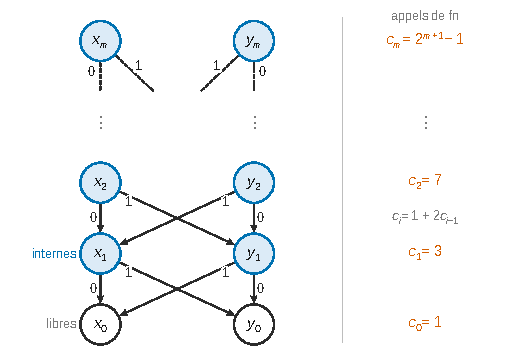
\includegraphics{figures/q10-famille-etages.pdf}
\caption*{Figure 2 --- Famille de graphes de la Q10 : deux sommets par étage, arcs
vers l'étage inférieur, et nombre d'appels de fn par étage}
\end{figure}

Ce graphe est acyclique, car les arcs vont de l'étage \(i\) à l'étage \(i-1\). Son degré sortant est au plus 2, et il n'a pas d'arc multiple. Ce n'est pas un arbre : chaque sommet de l'étage \(i-1\) est la cible de deux arcs, ce qui fait doubler le nombre d'appels à chaque étage. Par symétrie, \(C(x_i)=C(y_i)\), que l'on note \(c_i\). On a

\equationajustee{\begin{aligned}
c_0&=1,\\
c_i&=1+2c_{i-1}\ \text{ pour } 1\le i\le m,\\
c_i+1&=2(c_{i-1}+1),\\
c_m&=2^{m+1}-1.
\end{aligned}}

Comme \(m+1=n/2\) :

\equationajustee{\boxed{C(x_m)=2^{n/2}-1}}

Chaque appel coûte au moins une opération élémentaire. \textbf{La complexité dans le pire cas de \texttt{fn} est donc au moins exponentielle en le nombre de sommets.}

Variante plus simple, si l'on accepte deux arcs vers le même sommet (la représentation par listes le permet) : une chaîne \(s_0,\dots,s_{n-1}\) où \texttt{G{[}s\_i{]}\allowbreak{}\ =\allowbreak{}\ {[}s\_\{i+1\},\allowbreak{}\ s\_\{i+1\}{]}\allowbreak{}} pour \(i<n-1\), et \(s_{n-1}\) libre. Elle donne \(2^n-1\) appels pour \(n\) sommets.

\hypertarget{question-11}{%
\subsection{Question 11}\label{question-11}}

On mémoïse le résultat par sommet dans un dictionnaire. La présence est testée au début de \texttt{aux}, et le cas de base est mémoïsé comme les autres :

\begin{lstlisting}[language=Python]
def fn_efficace(s):
    memo = {}

    def aux(x):
        if x not in memo:
            if len(G[x]) == 0:          # libre
                memo[x] = x
            elif len(G[x]) == 1:        # lié
                memo[x] = aux(G[x][0])
            else:                       # interne
                memo[x] = (aux(G[x][0]), aux(G[x][1]))
        return memo[x]

    return aux(s)
\end{lstlisting}

\emph{Correction.} \texttt{aux} suit exactement la définition de \(\mathrm{fn}\). La valeur mémorisée pour \(x\) est \(\mathrm{fn}(x)\), et \texttt{aux} termine par Q9.

\emph{Complexité.} Le calcul et l'affectation de \texttt{memo{[}x{]}} s'exécutent au plus une fois par sommet. Hors appels récursifs, ils coûtent \(O(1)\) : tests, accès au dictionnaire, construction d'un couple.

Un couple ne contient que deux références vers des valeurs déjà construites : les sous-termes sont \textbf{partagés} et ne sont pas recopiés. Chaque calcul de \texttt{memo{[}x{]}} lance au plus deux appels, donc le nombre total d'appels à \texttt{aux} est au plus \(1+2|S|\). \textbf{La complexité est \(O(|S|)\).}

\hypertarget{question-12}{%
\subsection{Question 12}\label{question-12}}

Si \(s\) est libre, \(T(s)=1\), car le seul chemin est le chemin vide. Sinon, un chemin issu de \(s\) qui aboutit à un sommet libre commence par l'un des arcs sortants de \(s\). Cela donne une partition des chemins comptés, d'où

\equationajustee{T(s)=\sum_{s\to t}T(t).}

La récursion termine par Q9. Le sujet n'exige pas d'efficacité, et la récursion directe suffirait. On mémoïse quand même, pour un coût linéaire :

\begin{lstlisting}[language=Python]
def taille(s):
    memo = {}

    def aux(x):
        if x not in memo:
            if len(G[x]) == 0:
                memo[x] = 1
            else:
                total = 0
                for y in G[x]:
                    total = total + aux(y)
                memo[x] = total
        return memo[x]

    return aux(s)
\end{lstlisting}

Vérification sur la figure 1 : \(T(a)=T(c)+T(d)=2+2=4\), et \(T(W)=T(Z)=1\). \textbf{Complexité \(O(|S|)\)} grâce à la mémoïsation. Sans elle, le coût serait exponentiel sur l'exemple de Q10.

\hypertarget{question-13}{%
\subsection{Question 13}\label{question-13}}

Soit \(H\) une extension de \(G\). Une extension n'ajoute d'arcs qu'aux sommets libres. Donc \(c\) reste interne dans \(H\), avec \(c_0=X\) et \(c_1=Y\) :

\equationajustee{{\mathrm{fn}}_H(c)=\big({\mathrm{fn}}_H(X),\ {\mathrm{fn}}_H(Y)\big).}

\(H\) vérifie A1 et A5, donc Q9 s'applique à \(H\) : les formes normales dans \(H\) sont des termes finis. On définit leur taille par \(|v|=1\) pour un sommet et \(|(\alpha,\beta)|=1+|\alpha|+|\beta|\) pour un couple. On a donc

\equationajustee{|{\mathrm{fn}}_H(c)|=1+|{\mathrm{fn}}_H(X)|+|{\mathrm{fn}}_H(Y)|>|{\mathrm{fn}}_H(X)|.}

Ainsi \({\mathrm{fn}}_H(c)\neq{\mathrm{fn}}_H(X)\), quelle que soit l'extension \(H\), que \(X\) y reste libre ou y devienne lié. \textbf{Le problème \(\{(c,X)\}\) n'a pas de solution.}

\hypertarget{question-14}{%
\subsection{Question 14}\label{question-14}}

Ligne 17, on complète par :

\begin{lstlisting}[language=Python]
        elif len(G[s]) == 0:
            if s != t and not lier(s, t):
                return False
\end{lstlisting}

\emph{Justification.} Cette branche n'est atteinte que si \(s\) est libre et \(t\) n'est pas lié, c'est-à-dire \(t\) libre ou interne.

En effet, les cas « \(t\) lié » et « \(s,t\) internes » sont traités avant. La branche \texttt{else} ramène le cas « \(s\) interne, \(t\) libre » à celui-ci par T1.

\texttt{unif} ne modifie \(G\) que par \texttt{lier}, qui préserve A1--A4 (Q7). Les invariants sont donc vrais à chaque appel de \texttt{lier}, et Q5 s'applique : \texttt{lier(s,\ t)} ajoute l'arc \(s\to t\) si et seulement si \(t\not\rightsquigarrow s\).

\begin{itemize}
\tightlist
\item
  Si \(s=t\), la paire est satisfaite par toute extension. On la retire simplement de \(P\). Le test \texttt{s\ !=\ t} est indispensable : \texttt{lier(s,\ s)} renverrait \texttt{False}, puisque \(s\rightsquigarrow s\).
\item
  Si \(s\neq t\), on est dans les hypothèses de T4 : \(P\) a une solution si et seulement si \(P'\) en a une qui contient l'arc \(s\to t\).

  \begin{itemize}
  \tightlist
  \item
    Si \(t\rightsquigarrow s\), aucune extension ne contient \(s\to t\), car elle contient \(G\) et elle est acyclique. \texttt{lier(s,\ t)} renvoie \texttt{False} : \(P\) n'a pas de solution.
  \item
    Sinon, \texttt{lier} ajoute l'arc \(s\to t\), étiqueté 0 puisque \(s\) était libre. Les extensions du nouveau \(G\) sont exactement les extensions de l'ancien qui contiennent \(s\to t\). On poursuit la boucle avec \(P'\), déjà privé de \((s,t)\) par \texttt{P.pop()}.
  \end{itemize}
\end{itemize}

On ne renvoie pas le résultat de \texttt{lier} quand il vaut \texttt{True} : la boucle doit continuer à traiter les autres paires de \(P\). Par exemple, sur la figure 1, \texttt{unif(\allowbreak{}{[}(\allowbreak{}\textquotesingle{}c\textquotesingle{},\allowbreak{}\ \textquotesingle{}X\textquotesingle{})\allowbreak{},\allowbreak{}\ (\allowbreak{}\textquotesingle{}Y\textquotesingle{},\allowbreak{}\ \textquotesingle{}Z\textquotesingle{})\allowbreak{}{]}\allowbreak{})\allowbreak{}} lie \texttt{Y} à \texttt{Z}, puis doit encore découvrir que \((c,X)\) n'a pas de solution (Q13) et renvoyer \texttt{False}.

\hypertarget{question-15}{%
\subsection{Question 15}\label{question-15}}

On renvoie les arcs qui violent A3 ou A4. Les deux invariants sont vérifiés si et seulement si le résultat est vide.

\begin{lstlisting}[language=SQL]
SELECT a.source, a.cible
FROM arcs AS a
JOIN sommets AS s ON s.id = a.source
JOIN sommets AS t ON t.id = a.cible
WHERE s.époque > t.époque
   OR (s.époque = t.époque AND s.sortie < t.sortie);
\end{lstlisting}

La violation de A3 s'écrit \(\texttt{\text{époque}}[s]>\texttt{\text{époque}}[t]\). La négation de l'implication A4 s'écrit : époques égales \textbf{et} \(\texttt{sortie}[s]<\texttt{sortie}[t]\). On peut aussi remplacer la première ligne par \texttt{SELECT\ COUNT(*)}, qui doit valoir 0.

\hypertarget{question-16}{%
\subsection{Question 16}\label{question-16}}

\textbf{Lemme.} Il existe deux sommets \(s\neq t\) tels que \(\mathrm{fn}(s)=\mathrm{fn}(t)\) si et seulement si l'une des conditions suivantes est remplie :

\begin{itemize}
\item
  \begin{enumerate}
  \def\labelenumi{(\roman{enumi})}
  \tightlist
  \item
    \(G\) a un sommet lié ;
  \end{enumerate}
\item
  \begin{enumerate}
  \def\labelenumi{(\roman{enumi})}
  \setcounter{enumi}{1}
  \tightlist
  \item
    deux sommets internes distincts \(s,t\) ont les mêmes fils : \(s_0=t_0\) et \(s_1=t_1\).
  \end{enumerate}
\end{itemize}

\emph{Preuve.} Si \(s\) est lié, alors \(\mathrm{fn}(s)=\mathrm{fn}(s^*)\), et \(s\neq s^*\) par acyclicité. Si \(s,t\) sont internes et ont les mêmes fils, alors

\equationajustee{\mathrm{fn}(s)=\big(\mathrm{fn}(s_0),\mathrm{fn}(s_1)\big)=\mathrm{fn}(t).}

Réciproquement, on suppose qu'aucun sommet n'est lié et qu'il existe des paires \(s\neq t\) avec \(\mathrm{fn}(s)=\mathrm{fn}(t)\). On en choisit une qui minimise \(N(s)\) (Q9). La forme normale d'un sommet libre est un sommet, celle d'un sommet interne est un couple.

\begin{itemize}
\tightlist
\item
  Si \(s\) ou \(t\) est libre, les deux le sont, et \(s=\mathrm{fn}(s)=\mathrm{fn}(t)=t\), ce qui est exclu.
\item
  Les deux sommets sont donc internes, avec \(\mathrm{fn}(s_0)=\mathrm{fn}(t_0)\) et \(\mathrm{fn}(s_1)=\mathrm{fn}(t_1)\).
\item
  Si \(s_0\neq t_0\), la paire \((s_0,t_0)\) conviendrait avec \(N(s_0)<N(s)\), ce qui contredit la minimalité. Donc \(s_0=t_0\), et de même \(s_1=t_1\) : on est dans le cas (ii). \(\square\)
\end{itemize}

\begin{figure}[H]
\centering
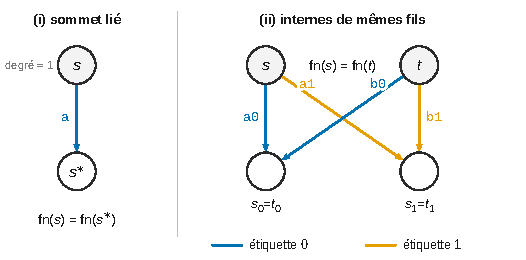
\includegraphics{figures/q16-temoins-locaux.pdf}
\caption*{Figure 3 --- Les deux motifs cherchés par la requête de la Q16 : sommet
lié et sa cible, deux internes de mêmes fils, arcs nommés par leurs
alias SQL}
\end{figure}

Il suffit donc de chercher ces deux motifs, sans calculer de forme normale. La requête suivante renvoie une telle paire, ou un résultat vide s'il n'en existe pas :

\begin{lstlisting}[language=SQL]
SELECT a.source, a.cible                      -- (i) un sommet lié et sa cible
FROM arcs AS a
JOIN sommets AS s ON s.id = a.source
WHERE s.degré = 1
UNION
SELECT a0.source, b0.source                   -- (ii) deux internes de mêmes fils
FROM arcs AS a0
JOIN arcs AS b0 ON b0.cible = a0.cible AND b0.étiquette = 0
JOIN arcs AS a1 ON a1.source = a0.source AND a1.étiquette = 1
JOIN arcs AS b1 ON b1.source = b0.source AND b1.étiquette = 1
                AND b1.cible = a1.cible
WHERE a0.étiquette = 0 AND a0.source < b0.source
LIMIT 1;
\end{lstlisting}

La présence d'un arc d'étiquette 1 garantit que les sommets de la seconde partie sont internes. La condition \texttt{a0.source\ \textless{}\ b0.source} impose \(s\neq t\). Dans la première partie, \(s\neq s^*\) par acyclicité.

\textbf{Toute ligne renvoyée vérifie \(s\neq t\) et \(\mathrm{fn}(s)=\mathrm{fn}(t)\), et le lemme garantit qu'une ligne est renvoyée dès qu'une telle paire existe.} Sur la figure 1, la requête renvoie \((W,Z)\).

\end{document}
